
\chapter{Case studies}
\label{casestudies}

\section{Case Study 1: Michael Giacchino}

Michael Giacchino (1967). website:\url{http://www.michaelgiacchinomusic.com/}. Note well his dedication to his education. He received a very thorough grounding in film, art and music. His major career boost came when he began writing for games including the well known \textit{Medal of Honor} series. He then teamed up with J.J.Abrams and wrote for a number of TV series. And through this collaboration he wrote for \textit{Star Trek} and \textit{Star Trek Into Darkness}.

His collaboration with Brad Bird have included \textit{The Incredibles}, \textit{Ratatouille}. His collaboration with Matt Reeves resulted in a score for \textit{Dawn of the Planet of the Apes}. His collaboration with Pete Doctor resulted in a score for \textit{UP}. His collaboration with Andrew Stanton resulted in a score for \textit{John Carter}.

\subsection{John Carter}
\begin{itemize}
\item Science fiction but with a Wild West slant.   
\item Horn theme. A lot of music backing the picture from simple drones to pulsing percussion.  
\item A three note theme. Open fifth (chord I to IVmin)
\item Use of Ostinati and heavy reliance upon strings.
\item Similarities with Star Trek especially in the love theme (around 1:15:00 and 1:17:30)
\end{itemize}

\subsection{Star Trek}
\begin{itemize}
\item orchestration
\item incorporation of old themes
\item the `strange harmony'
\end{itemize}

\section{Case Study 2: Bernard Herrmann}
\begin{itemize}
\item \href{http://www.bernardherrmann.org/}
{The Society for the Appreciation of the Music of Bernard Hermann}
\item Much to be learned from \textit{Bernard Herrmann's Vertigo} (a film score handbook) by David Cooper \citep{cooper2001bernard}
\item \textit{Vertigo} is on Box of Broadcasts. 
Herrmann's best film work prior to Vertigo was perhaps \textit{Citizen Kane} but really Herrmann had a foot in both camps: concert music and film scores.  Early association with Aaron Copland. Early recruitment into the service music industry and radio perhaps shifted Herrmann's path (which was to follow in Copland's footsteps). Herrmann got to know Orson Welles during this time and this led to the commission for \textit{Citizen Kane} - apparently a fee of \$10,000. Early employment of leitmotive for character and scene. Herrmann pre-dated the Barron's sci-fi world of electronic sound with a score featuring electronic instruments. In 1951 he scored the music for Robert Wise's film \textit{The Day The Earth Stood Still}. Later he was to go on to score \textit{Taxi Driver}. Interesting to compare the change in scoring. Herrmann met Hitchcock in 1955 and a number of film scores followed. \textit{Vertigo} began filming in 1957.

Cooper \citeyearpar{cooper2001bernard} numbers Herrmann's influences as: Wagner (chromatic harmony); Puccini (diatonic \textit{bel canto}); Schoenberg \textit{Klangfarbenmelodie}. Also Copland, Stravinsky and Delius. 

\subsection{Example of melody writing in \textit{Vertigo}}

All score examples are from Cooper's text \citeyearpar{cooper2001bernard}

\begin{figure}[H]
\centering
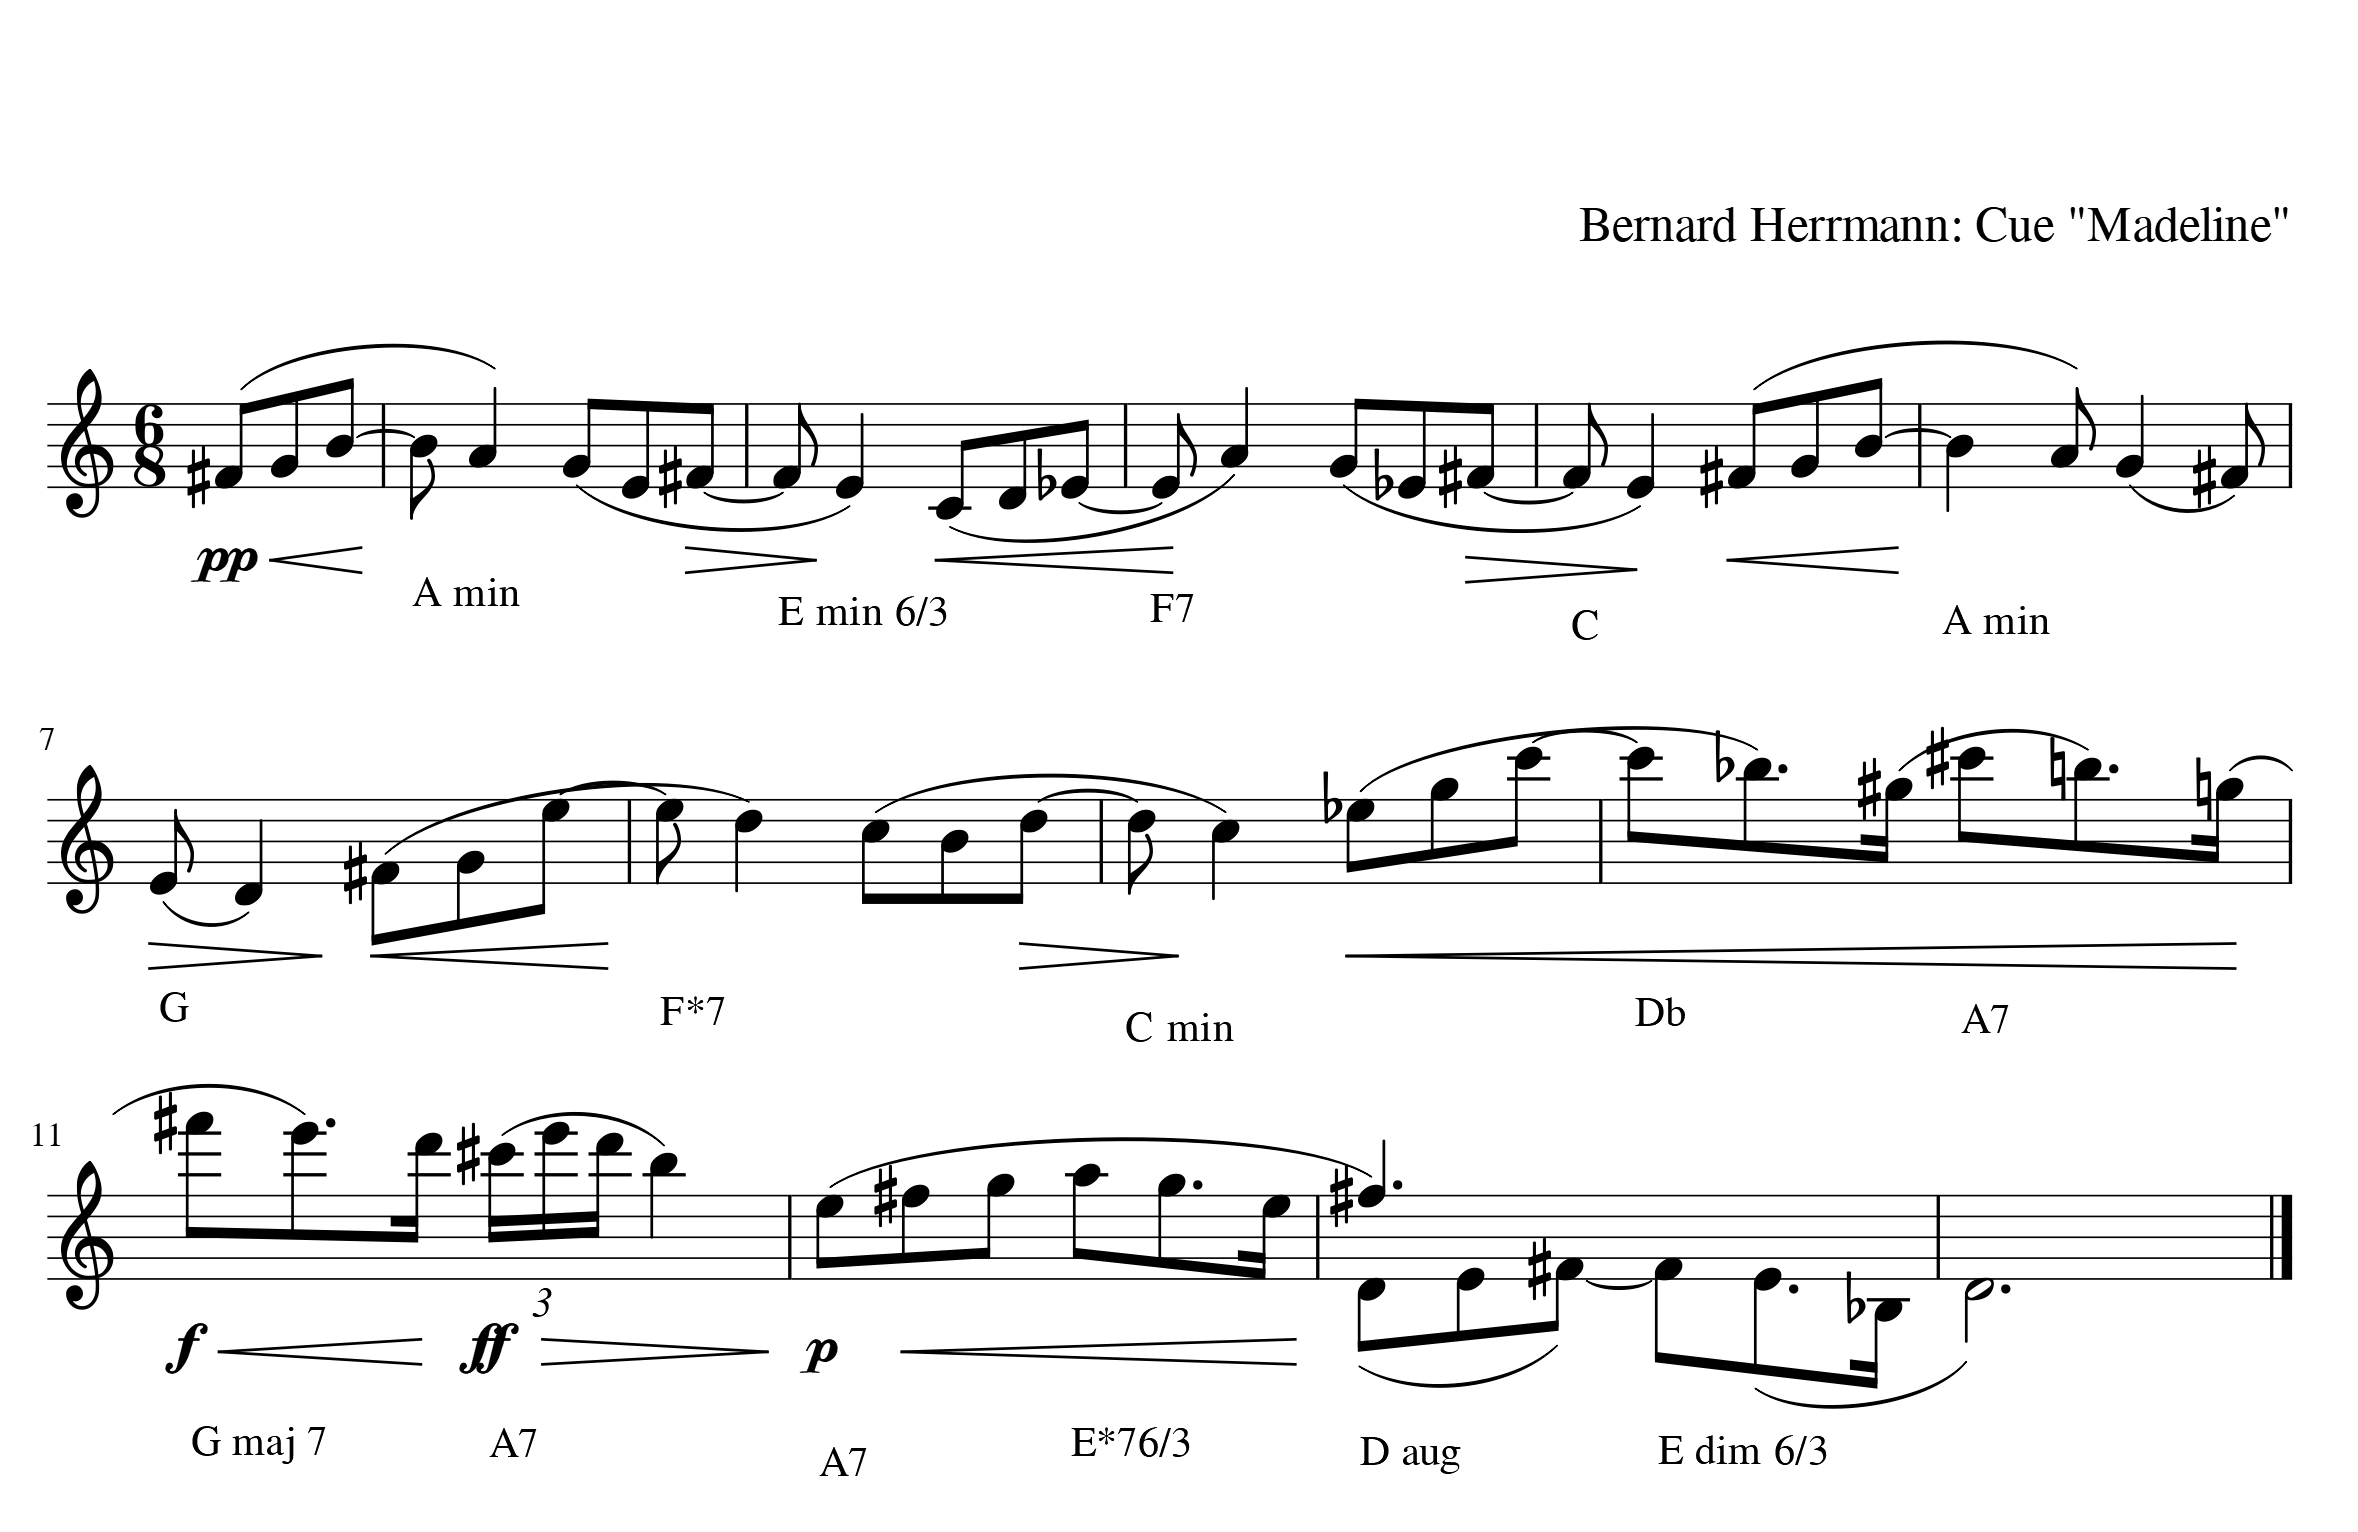
\includegraphics[scale=0.8]{herrmann-madeline}\caption{Hermann: Madelline theme}
\label{fig:Hermann-madeline theme}
\end{figure}

Herrmann remarked, `I don't think that the leitmotif is the only way of writing a film score, because I think you can do it using the operatic principles of Verdi where each number is separate and not derived from others'. However in both \textit{Citizen Kane} and \textit{Vertigo}, leitmotif is used extensively. 

Key features of \textit{Vertigo} (and its music) are mirror images, spirals and obsession. 

\begin{figure}[H]
\centering
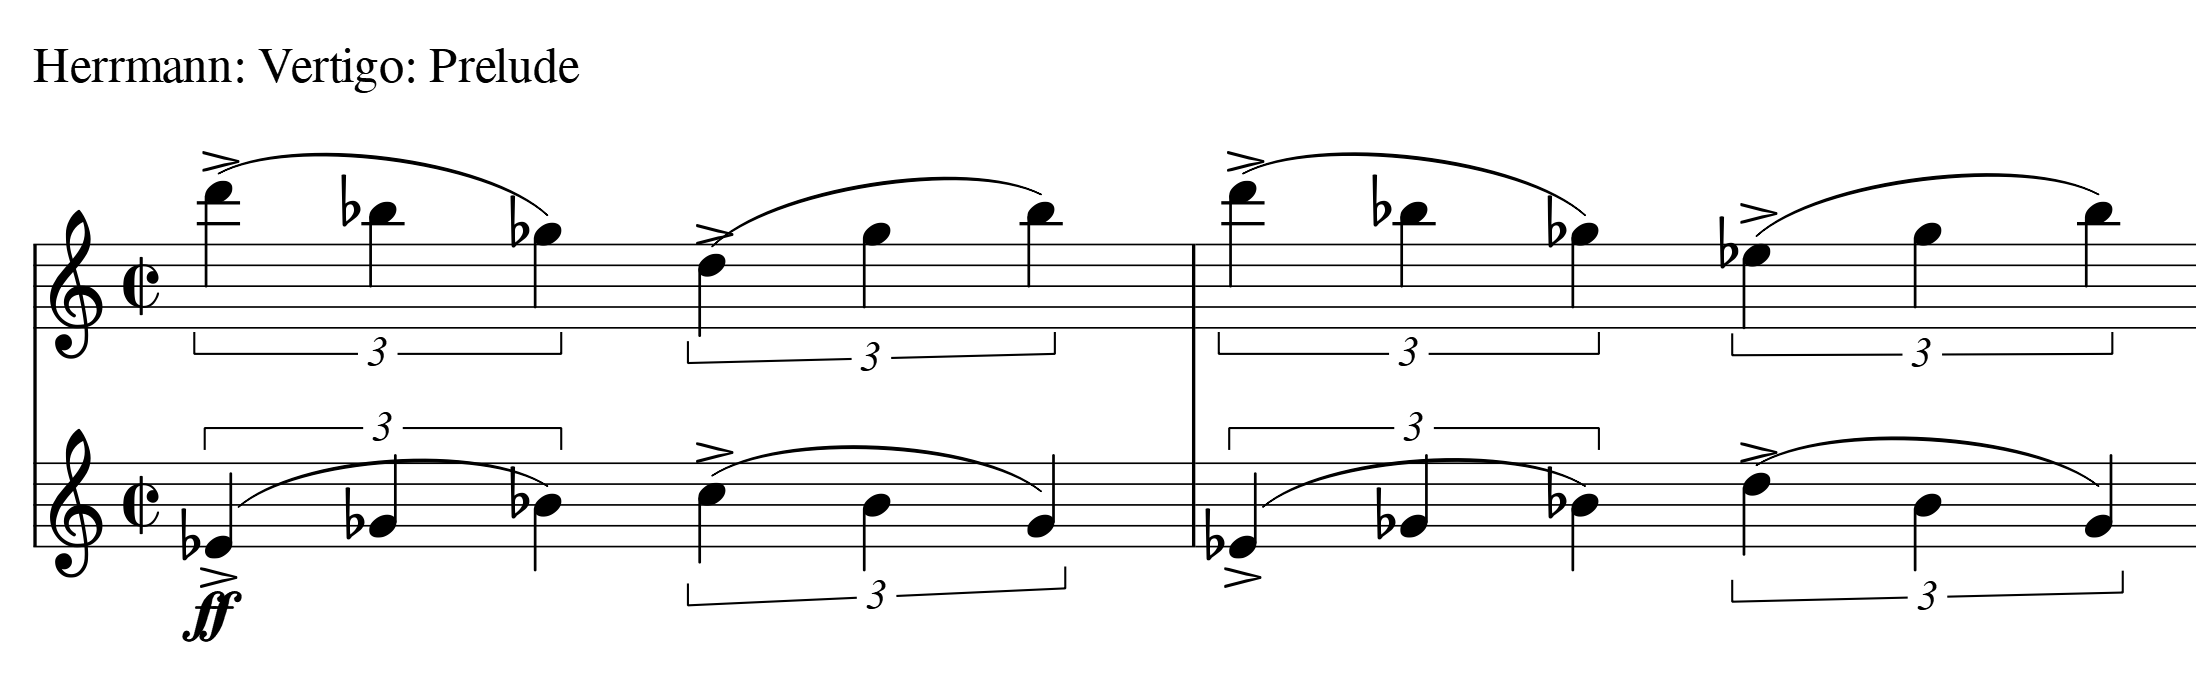
\includegraphics[scale=0.8]{herrmann-prelude}\caption{Hermann: Prelude}
\label{fig:Hermann-prelude}
\end{figure}

This passage demonstrates the mirror and obsession quite nicely. Much of Herrmann's work before and after Vertigo was heightened by a superb sense of orchestration. Check the music for \textit{Psycho}, \textit{The Day the Earth Stood Still} and \textit{Citizen Kane}. 
\end{itemize}




\section{Case Study 3: Stanley Kubrick}
Ligeti's music is closely linked to the films of Stanley Kubrick. 
\begin{itemize}
\item 2001: A Space Odyssey
\begin{itemize}
\item Atmosphères (StarGate sequence and other places) 
\item Lux Aeterna (for the moon-bus scene en route to the TMA-1 monolith)
\item Requiem (Kyrie linked to the black monolith)
\item Aventures (closing scenes)
\item There are small recurrences in the film 2010.
\end{itemize}
\item The Shining uses small portions of Lontano for orchestra alongside music in a similar vein by Penderecki (Utrenja, De Natura Sonoris No.1 and No.2, and Polymorphia)
\end{itemize}

\section{Case Study 4: Jerry Goldsmith}
Influences include Bela Bartok, Igor Stravinsky and Arnold Schoenberg. 
\begin{itemize}
\item Logan's Run
\item Planet of the Apes
\end{itemize}
Planet of the Apes has been extensively analysed by John O'Callaghan \citep{o2015simians}. Have a look at the 12 note row.

\begin{figure}[H]
\centering
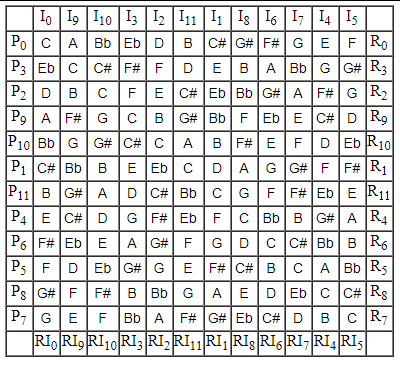
\includegraphics[scale=2.0]{potarow} \caption{Planet of the Apes: Row generator}
\label{fig:potarow}
\end{figure}

and as it appears as the `Main Title' (though never really appearing like this again but strongly suggesting that this is a 12 note motif).

\begin{figure}[H]
\centering
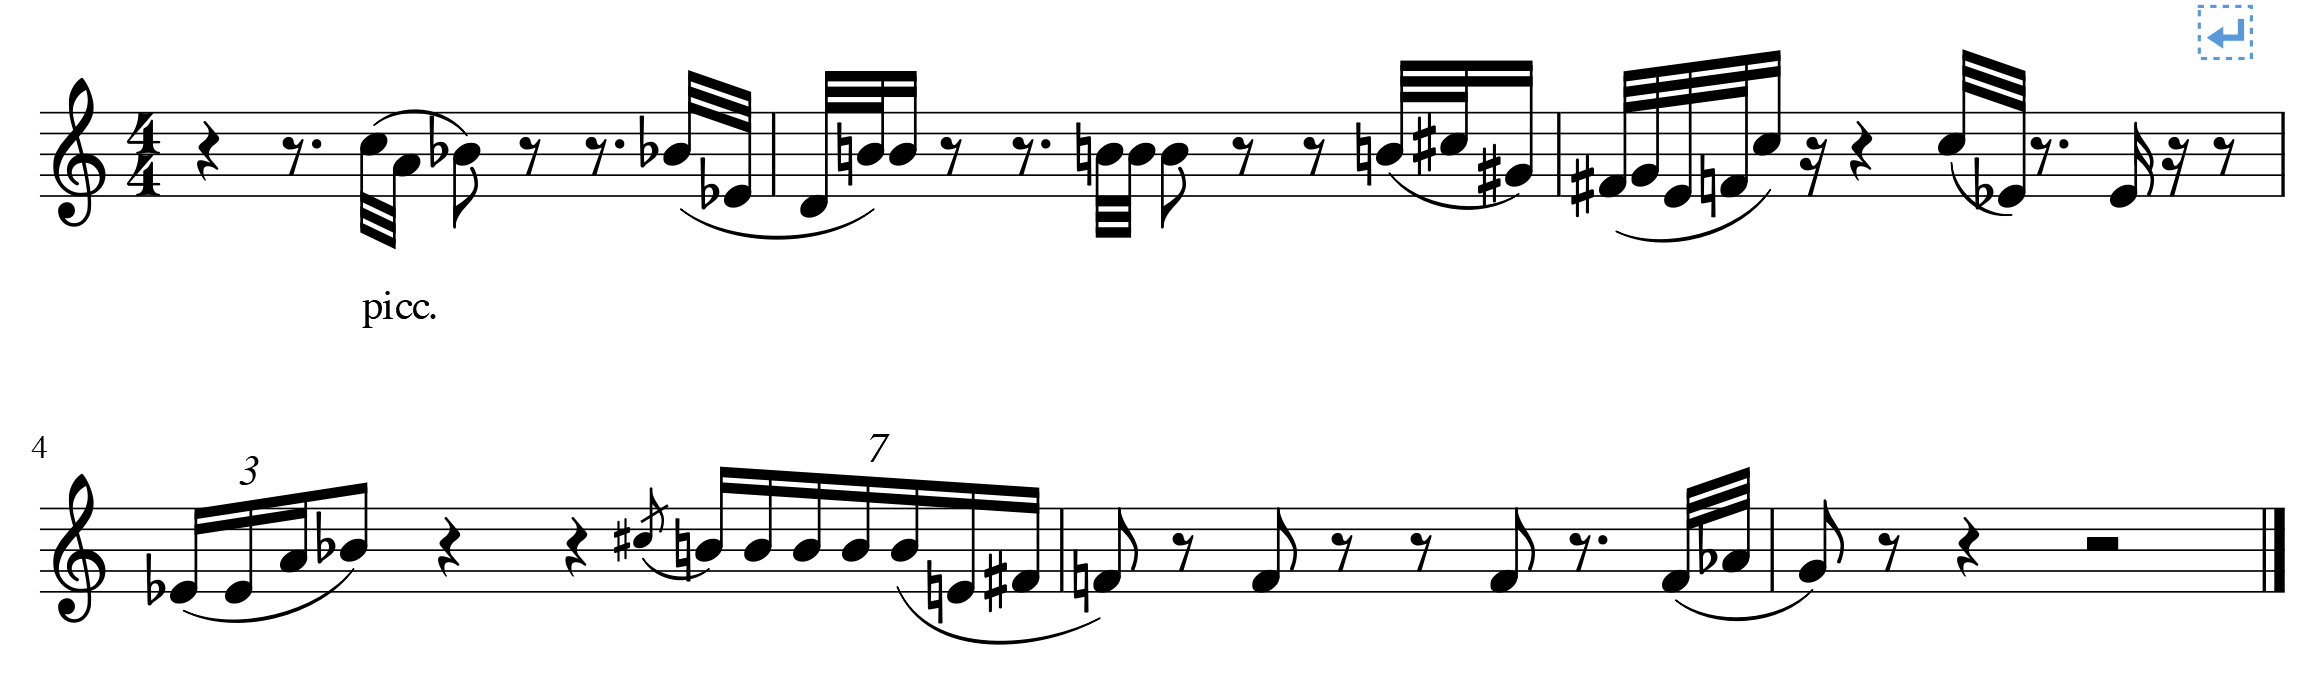
\includegraphics[scale=0.8]{potamaintheme}\caption{Planet of the Apes: Main Title}
\label{fig:potamaintheme}
\end{figure}



